\documentclass[17pt]{extarticle}
\usepackage{amsmath, amssymb}
\usepackage{nccmath}
\usepackage[a4paper, total={8in, 11.38in},top=2mm,left=27mm,bottom=2mm,right=2mm]{geometry}

\usepackage{tikz}

\usepackage{titlesec}
\titleformat{\section}
{\normalfont\normalsize\bfseries}{\thesection}{1em}{}

\titleformat{\subsection}
{\normalfont\normalsize\bfseries}{\thesection}{1em}{}

\usepackage{mathtools}

\usepackage{tasks}

\begin{document}

\noindent
\begin{fleqn} 

%%%%%%%%%%%%%%%%%%%%%%%%%%%%%%%%%%%%%%%%%%%%%%%%%%%%%%%%%%%%%%%%

\section{Question} 

$\begin{aligned}[t] 
\text{If \ } \int_{a}^{b} x^2 dx = \frac{2}{3} 
\text{\quad and\quad} 
\int_{a}^{b} x^3 dx = 0 
\text{\quad then\quad}
\int_{a}^{b} x^4 dx = \cdots
\end{aligned}$

\settasks{counter-format={(tsk[a])},label-offset=1em}
\begin{tasks}(4)
  \task $\dfrac{-2}{5}$ 
  \task $\dfrac{-2}{5}$ 
  \task $\dfrac{-2}{5}$ 
  \task $\dfrac{-2}{5}$
\end{tasks}
%----------------------------------------
\subsection*{Answer}
Let  'x'  be the side of a square base and 'h' be the height of the box.\
$\therefore$ Total surface area = $x^2+4h = 300\,cm^2$
%%%%%%%%%%%%%%%%%%%%%%%%%%%%%%%%%%%%%%%%%%%%%%%%%%%%%%%%%%%%%%%%

\section{Question}
The slant height of a right circular cone is 3 cm. Find the height of cone, if its volume is the greatest.

%----------------------------------------

\subsection*{Answer}
Let  r  and x  be the base-radius and the height of the cone respectively. Then the volume f(x) of the cone is given by

\begin{equation} \nonumber
\begin{alignedat}{4}
f(x) &= \frac{1}{3}\pi r^2x\\
&= \frac{\pi}{3}(3^2-x^2)x\\
&= \frac{\pi}{3}(9x - x^3)\\
\therefore f'(x) &=  \frac{\pi}{3}(9 - 3x^2)\\
\end{alignedat}
%\vrule
\quad\quad\quad
\begin{alignedat}{4}
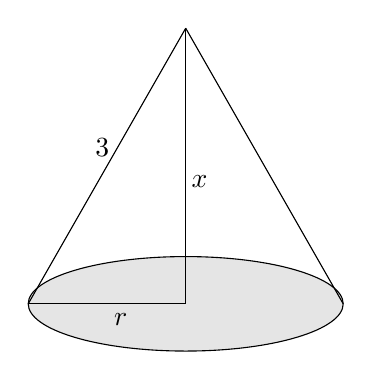
\begin{tikzpicture}
\filldraw[fill=gray!20](0,0) ellipse (2cm and 0.6cm);
\draw (0,0) -- node[below] {\ \ \ $x$}(0,3.5);
\draw (0,0)  -- node[below] {\ \ \ $r$} (-2,0);
\draw  (-2,0) --node[above] {3\ \ }(0,3.5);
\draw  (2,0) -- (0,3.5);
\end{tikzpicture}\\\\
\end{alignedat}
\end{equation}
\begin{equation} \nonumber
\begin{alignedat}{4}
& Now\ f'(x) = 0\ gives\\
& \frac{\pi}{3}(9x - x^3)=0\\
& \therefore \ 3x^2=9\\
& \therefore x = \sqrt{10}
\end{alignedat}
\quad
\vrule
\quad
\begin{alignedat}{4}
& Also\ \ f''(x) =-6x\\
& \therefore\ \ f''(\sqrt{3})=-6\sqrt{3}<0\\
& \therefore \ \ By\ second\ derivative\ test\\
& Volume \ f\ is maximum\ at\ x=\sqrt{3}
\end{alignedat}
\end{equation}
%%%%%%%%%%%%%%%%%%%%%%%%%%%%%%%%%%%%%%%%%%%%%%%%%%%%%%%%%%%%%%%%


\end{fleqn}
\end{document} 